\hfill\break
\justifying
Integrando el escalado en grises, inversión de los colores y los métodos manuales y automáticos de umbralado, se tratan a fondo los métodos de umbralado automático únicamente, y aunque la funcionalida de inversión de colores es una función reciente, su implementación es tan sencilla como la negación por bit de su valor en la imagen. Otro enfoque más sencillo consiste en restar a 255 el valor actual de cada pixel.

\subsection*{Método de Kapur}
	\hfill\break
	\justifying
	Esta técnica de umbralado se utiliza cuando en una imagen se encuentran 2 tendencias de los niveles en escalas de grises, una perteneciente al fondo y la otra al objeto, para esto los objetos deben tener un buen contraste respecto al fondo.
	
	\hfill\break
	\justifying
	La umbralización automática de Kapur, se centra en encontrar un valor para el umbral \textit{u}, tal que la división dicotómica de clases para una imagen basándose en los valores de grises de los píxeles según su histograma, seá la maximización de la medida de la información utilizando le ecuación de la entropía como medida de la información.
	
	\hfill\break
	\justifying
	Se define a la entropía de la imagen completa como:
	\begin{equation*}
		H_T = -\sum_{r=0}^{L-1} p_r ln(p_r)
	\end{equation*}
	
	\hfill\break
	\justifying
	La información de las 2 clases es: $I(C_1,C_2)=H_{C_1}(u)+H_{C_2}(u)$. La definición de la entropía de cada clase son las ecuaciones:
	{\large \begin{equation*}
		\begin{array}{r l l}
			H_{C_1}(u)= & -\overset{u}{\underset{r=0}{\sum}}\frac{p_r}{p(C1)}ln\left( \frac{p_r}{p(C1)} \right) & = lnp(C_1)+\frac{H_u}{p(C1)}\\
			H_{C_2}(u)= & -\overset{L-1}{\underset{r=u+1}{\sum}}\frac{p_r}{1-p(C1)}ln\left( \frac{p_r}{1-p(C1)} \right) & = lnp(1-C_1)+\frac{H_t-H_u}{1-p(C1)}\\
		\end{array}
	\end{equation*}}
	Con $C_1$ como la probabilidad acumulada de los valores de los pixeles hasta el índice \textit{u}.

	\hfill\break
	\justifying
	Ambas ecuaciones como la suma de la información de cada clase se puede rescibir como un funcional:
	{\Large \begin{equation*}
		J_k(u) = ln[p(C_1)(1-p(C_1))]+\frac{H(u)}{p(C_1)}+\frac{H_T-H(u)}{1-p(C_1)}
	\end{equation*}}
	
	\hfill\break
	\justifying
	Buscando el valor de \textit{u} donde el funcional es máximo:
	{\Large \begin{equation*}
		u* = arg \underset{0 \leq u \leq L-1}{max} J_k(r)
	\end{equation*}}

	\hfill\break
	\justifying
	Su implementación se logra de manera sencilla utilizando las operaciones y propiedades que proveén los arreglos de la biblioteca numpy. Con funciones completamente vectorizadas, se determina el valor del umbral \textit{u} en muy poco tiempo y además con un código muy descriptivo parecido a las propias ecuaciones.
	
	\begin{lstlisting}[language=Python]
	def kapur_threshold(image):
		# Probability of each pixel value
		p,_ = histogram(image, bins=range(256), density=True)
		# Cumulative probabilities for C1 and C2
		c1 = p.cumsum(); c2 = 1.0 - c1
		# When the probabilities are 0 its changed to 1 so that it won't affect when used as divider
		c1[c1 <= 0] = 1; c2[c2 <= 0] = 1
		# Entropy of the image
		#   To avoid the case: ln(0)
		#   And as the entropy for each pixel values is p*ln(p)
		#   the values of p that are 0 are changed to 1 so when the entropy its
		#   applied the this pixel value won't affect the whole entropy
		#   ** The entropy of the whole image will be the last element of H_u
		p_1 = copy(p); p_1[p_1 == 0.0] = 1
		H_u = -(p_1*log(p_1)).cumsum()
		H_t = H_u[-1]
		# Functional
		#   Jk(u) = H_c1(u)+H_c2(u) = ln(c1*c2)+[H(u)/c1]+[(H_t-H(u))/c2]
		Jk = log(c1*c2)+(H_u/c1)+((H_t-H_u)/c2)
		return argmax(Jk)
	\end{lstlisting}

	\hfill\break
	\justifying
	Las pruebas del método de Kapur, otorgaron resultados mas bien malos para la umbralización de una imagen en clases dicotómicas, con valores de \textit{u} muy altos o muy bajos, para la imagen que se maneja. Se utilizan como ejemplos para este método 3 ímagenes sencillas obtenidas del banco de imágenes del propio Dr. Humberto Sossa, que describen objetos completamente negros de diferentes geometrías sobre un fondo color claro y unos palillos de paleta.
	
	\begin{figure}[!h]
		\begin{tabular}{cc}
			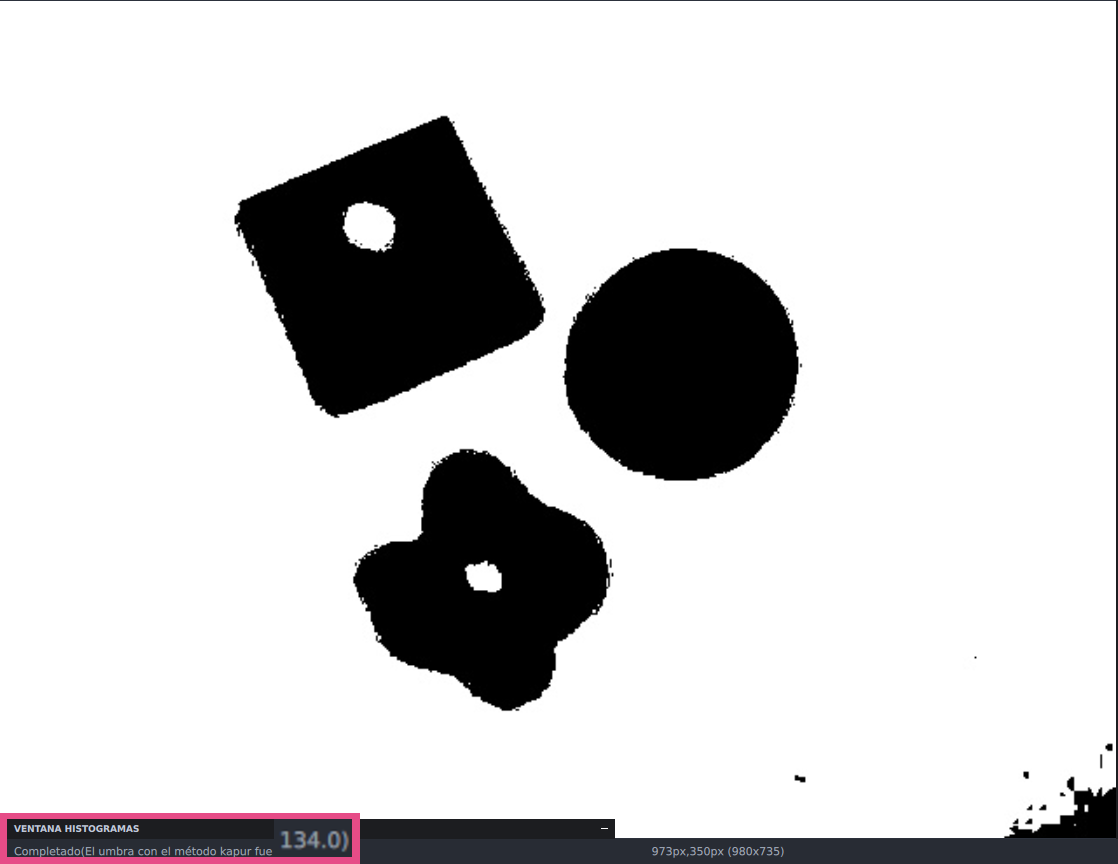
\includegraphics[width=9.5cm]{Imagenes/Kapur_1.png} & 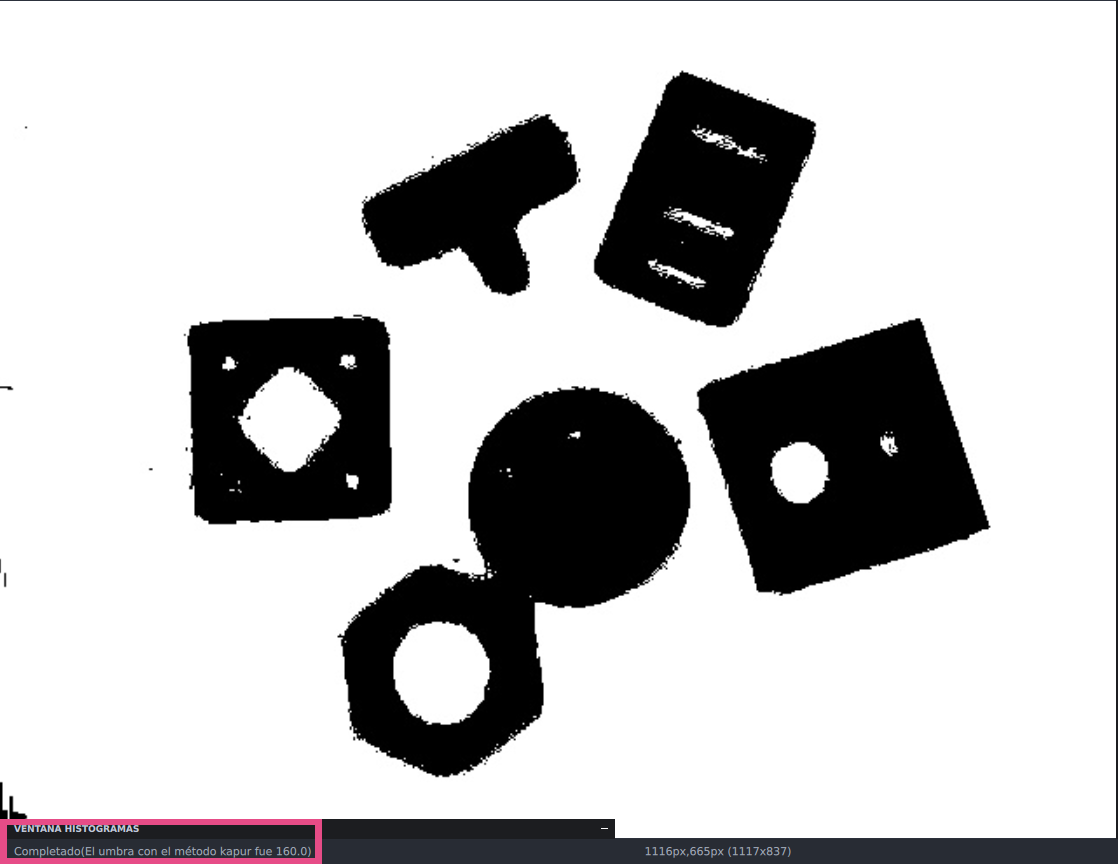
\includegraphics[width=9.5cm]{Imagenes/Kapur_2.png} \\
			\multicolumn{2}{c}{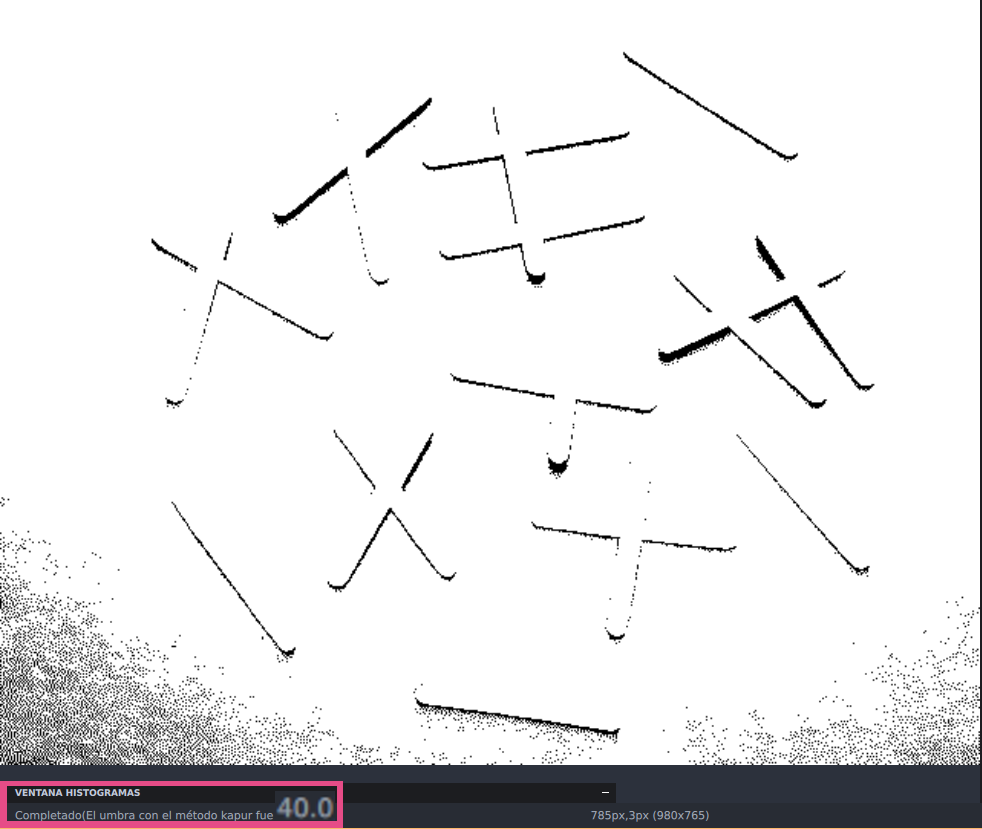
\includegraphics[width=10cm]{Imagenes/Kapur_3.png}}
		\end{tabular}
		\label{Kapur}
		\caption{Resultados obtenidos de la aplicación del método de Kapur para la umbralización automática. \\ 1) 3 objetos negros constrastados con un fondo claro. Se obtuvo un umbral muy grande(134) \\ 2) 6 objetos negros constrastados con un fondo claro. Se obtuvo un umbral muy grande(160) \\ 3) Palos de paleta claros con un fondo obscuro. Se obtuvo un umbral muy pequeño(40)}
	\end{figure}
	
\subsection*{Método de Cheng}
	\hfill\break
	\justifying
	Al igual que sucede con el método de Kapur, el método de Cheng se utiliza en el umbralado dicotómico, aunque es expandible a un entorno multiclase. En este trabajo se implementa de solo 2 modas.
	
	\hfill\break
	\justifying
	En esta técnica de binarización automática, los pixeles se suponen variables aleatorias de las que se puede calcular la correlación y a través de las distribuciones de probabilidad $C_1$ y $C_2$ se describe la cantidad de esta.
	
	\hfill\break
	\justifying
	Se recuerda que la correlación se puede calcular como:
	\begin{equation*}
		C(X) = -ln\sum_{r\geq1} p_r^2
	\end{equation*}
	Por lo tanto para cada distribución se define:
	\begin{equation*}
		\begin{aligned}
			G(u) = \sum_{r=1}^{u} p_r^2 \\
			G'(u) = \sum_{r=u+1}^{L-1} p_r^2 \\
		\end{aligned}
	\end{equation*}
	
	\hfill\break
	\justifying
	Como se intenta obtener la máxima correlación entre el objeto de interés y el fondo se realiza la suma de correlaciones para cada clase:
	\begin{equation*}
		CT(u) = C_{C_1}(u) + C_{C_2}(u)
	\end{equation*}
	Pudiendose calcular de la siguiente forma entonces:
	{\Large \begin{equation*}
		\begin{aligned}
			CT(u) = -ln\sum_{r=1}^{u} \left( \frac{p_r}{P_1(u)} \right)^2 -ln\sum_{r=u+1}^{L-1} \left( \frac{p_r}{1-P_1(u)} \right)^2 \\ = -ln[G(u)\times G'(u)]+2ln[P1(u)\times(1-P_1(u))]
		\end{aligned}
	\end{equation*}}
	
	\hfill\break
	\justifying
	Finalmente el umbral se obtiene de identificar el argumento del funcional que maximiza la correlación:
	{\Large \begin{equation*}
		u* = arg \underset{0\leq u \leq L-1}{max} CT(r)
	\end{equation*}}
	
	\hfill\break
	\justifying
	Muy similar a como sucede con Kapur, este método facilmente puede implementarse utilizanando operaciones y propiedades de los array de la biblioteca numpy, facilitando la operación, expresión y optimizando en operaciones pues estas son sumamente veloces.
	
	\begin{lstlisting}[language=Python]
	def cheng_threshold(image):
		# Frecuency of each pixel value
		_,p = histogram_no_image(image)
		# The filter for reducing 0 gets applied
		p = mean_filter(p)
		# Probabilities of each pixel value
		p = p/p.sum()
		# Cumulative probabilities for C1 and C2
		c1 = p.cumsum(); c2 = 1.0 - c1
		# Cumulative sum of the square of pixels probability and the complement
		G = (p**2).cumsum(); G_c = G[-1]-G
		# When the probabilities are 0 its changed to 1 so that it
		# won't affect when used inside the natural logarithm
		c1[c1 <= 0] = 1; c2[c2 <= 0] = 1
		G[G == 0] = 1; G_c[G_c == 0] = 1
		# Functional
		# CT(u) = C_c1(u)+C_c2(u) = -ln[G(u)xG'(u)]+2ln[P1(u)+P2(u)]
		CT = -log(G*G_c) + 2*log(c1*c2)
		return argmax(CT)
	\end{lstlisting}
	
	\hfill\break
	\justifying
	Las pruebas del método de Chen, al igual que el de Kapur, otorga resultados deficientes con valores de \textit{u} muy altos o muy bajos, lo que sugiere que se utilizen otro tipo de métodos como Kittler e Illinworth para la binarización automática de imagenes con 2 modas.
	
	\begin{figure}[!h]
		\begin{tabular}{cc}
			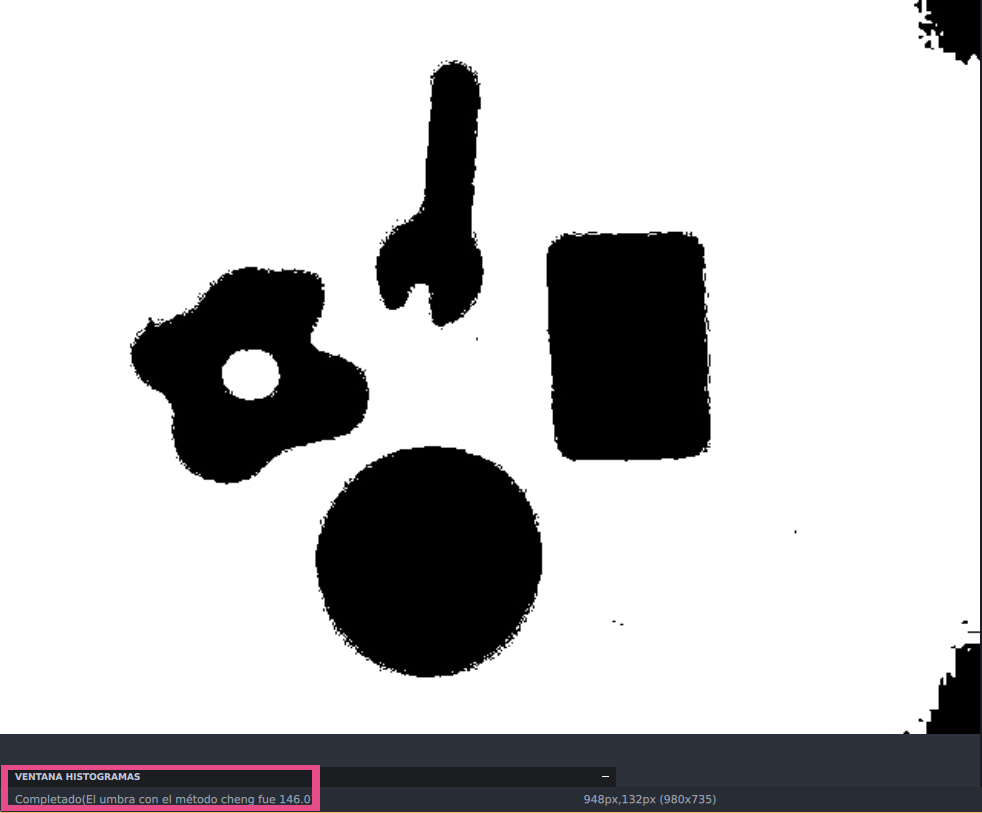
\includegraphics[width=10cm]{Imagenes/Cheng_1.png} & 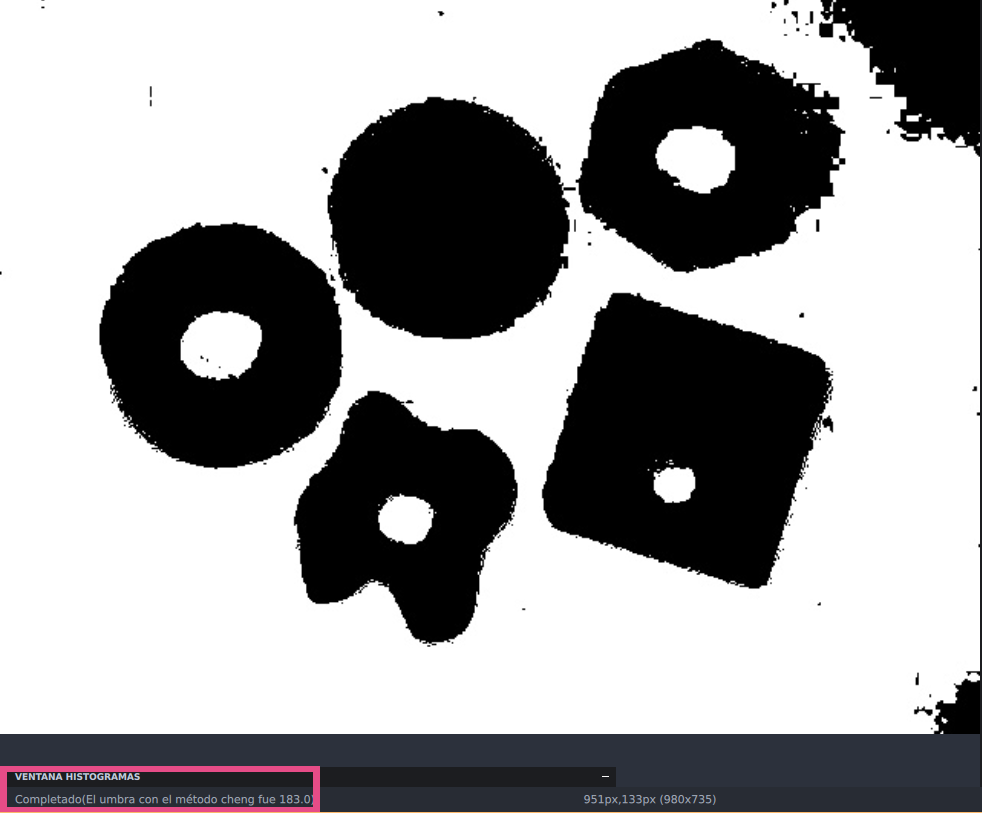
\includegraphics[width=9cm]{Imagenes/Cheng_2.png} \\
			\multicolumn{2}{c}{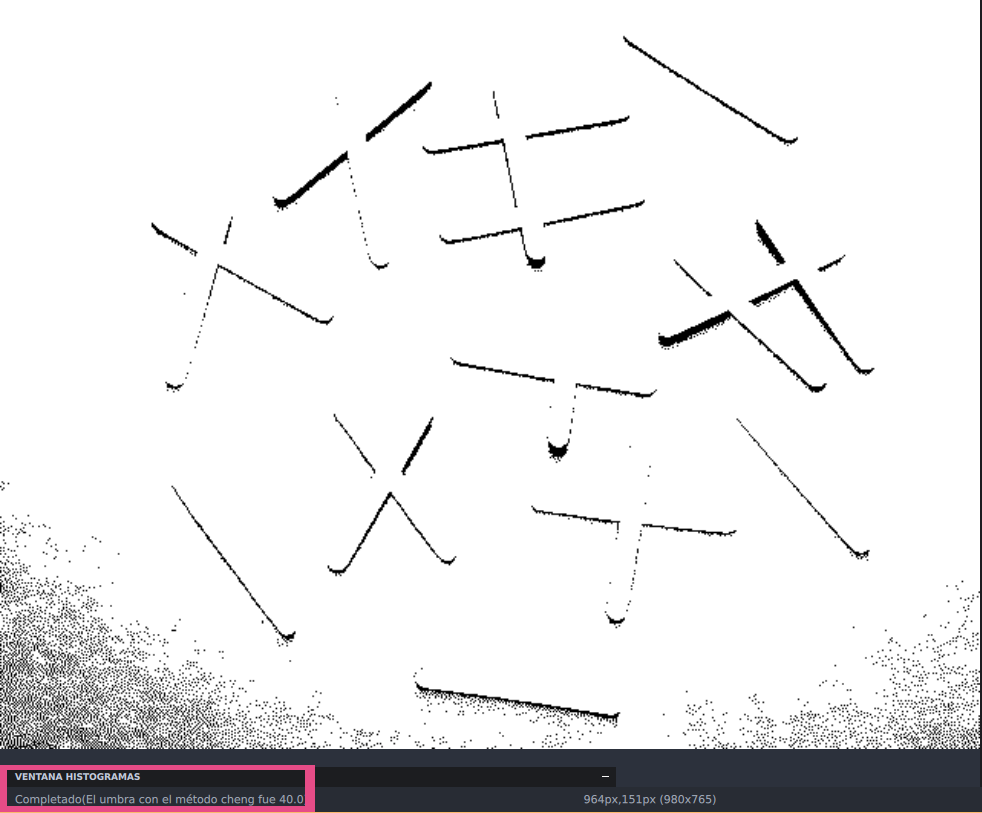
\includegraphics[width=11cm]{Imagenes/Cheng_3.png}}
		\end{tabular}
		\label{Cheng}
		\caption{Resultados obtenidos de la aplicación del método de Cheng para la umbralización automática. \\ 1) 4 objetos negros constrastados con un fondo claro. Se obtuvo un umbral muy grande(146) \\ 2) 5 objetos negros constrastados con un fondo claro. Se obtuvo un umbral muy grande(183) \\ 3) Palos de paleta claros con un fondo obscuro. Se obtuvo un umbral muy pequeño(40)}
	\end{figure}